\documentclass[12pt]{article}
\usepackage[utf8]{inputenc}

% --- General Setup --- %
\usepackage[margin=1in]{geometry}
\usepackage{float}
\usepackage{gensymb}
\usepackage{graphicx}

% --- Works Cited --- %
\usepackage[backend=biber,style=ieee,sorting=none]{biblatex}
\addbibresource{./sources.bib}

% --- Dummy Text --- %
\usepackage{lipsum}

% --- Introduction Formatting --- %
\renewcommand{\abstractname}{\Large{Introduction}}

% --- Tables --- %
\usepackage{multirow}
\usepackage{array}

\begin{document}
% ---------------- %
\begin{center}
    \large
    \textbf{GPGN 470A Term Project - Part II}
    
    \vspace{0.4cm}
    \large
    Engineering Literature Review of Delayed Doppler Map Instrumentation on board CYGNSS
    
    \vspace{0.4cm}
    Tyler Singleton
    
    \vspace{0.4cm}
    \today
    
    \vspace{0.9cm}
\end{center}
\begin{abstract}
    \normalsize
    \vspace{1em}
    
    The Cyclone Global Navigation Satellite Systems (CYGNSS) is a constellation consisting of eight micro-satellites originally intended to measure ocean wind speeds utilizing reflected GNSS signals from Global Positioning Satellites (GPS) \cite{NASA}. Recently, these reflected GNSS signals have shown potential to monitor global soil moisture (SM) levels as the signals are more sensitive to changes in SM than surface roughness and vegetation \cite{Global_SM}. The Delayed Doppler Mapping Instrument (DDMI) or SGR-ReSI is the primary instrumentation utilized to map the forward scattered GNSS signals \cite{DDMI_Overview}; it is capable of processing up to four reflections simultaneously and in real-time \cite{DDMI_Overview, DDMI_Summary}. In this paper, I will discuss an overview of the DDMI -- its history, capabilities, how it works, and display a delayed doppler map pulled from CYNGSS using level 1 data. 

\end{abstract}

% ---------------- %
\section{An Overview of Delayed Doppler Mapped Instrumentation}

In 2012, the University of Michigan was selected by NASA to lead the CYGNSS mission in monitoring ocean surface winds during topical storms and hurricanes \cite{SGR-ReSi_Application}. After the success of using GNSS Reflectometery (GNSS-R) to estimate geophysical parameters from the UK-Disaster Monitoring Constellation (DMC) mission, a partnership consisting of SwRI, NASA Ames, SST-US, and the US subsidiary of Surrey Satellite Technology (SSTL) formed to develop the DDMI for the CYGNSS mission \cite{SGR-ReSi_Application}. 

The DDMI is a unique instrument. It is capable of processing up to four reflected signals simultaneously and in real-time \cite{SGR-ReSi_Application}. This significantly reduces data storage which allows for the satellite to capture more reflections \cite{SGR-ReSi_Application}. However, for reflected GNSS signals to be considered useful, a bistatic configuration is necessary \cite{DDMI_Overview}. Thus, the DDMI comes with three antennas for processing reflected signals -- two for left hand circular polarized (LHCP) reflections facing the nadir direction, and one for the right hand circular polarized (RHCP) signals in the zenith direction for direct reference from GPS satellites \cite{DDMI_Overview}. They have of gain of 14 dB and 5 dB respectively \cite{DDMI_Overview}.

To calculate wind speeds of ocean surface winds, a delayed doppler map is necessary. The concept is to take the maximum spectral reflectance and average it with the mean noise floor \cite{GNSS_Signal_Properties}. The more rough the surface, the large the glistening zone, and thus higher the noise floor \cite{DDMI_Overview}. So distinguishing the reflected GNSS signal from background interference is fundamental to accurately estimating geophysical parameters, but reflected GNSS signals are weak \cite{SGR-ReSi_Application}, and this is a large challenge. Fortunately, GPS satellites use a pseudo-random carrier signal to modulate GNSS \cite{GNSS_Signal_Properties}. This modulation is what allows for the DDMI to pull out the weak GNSS signal, and why the bistatic satellite configuration is essential. The DDMI needs a direct reference to the GPS in order to decode the modulated signal and extract it from background noise and other GNSS reflections.

% ---------------- %
\section{Data Processing}

Since the DDMI processes reflected GNSS signals on board, there is no need to specific data processing software to clean the raw data. The satellite will transmit the rendered DDM as well as it GPS location and other physical and spacial parameters. The DDM can then be plotted with any Matlab library \cite{SGR-ReSi_Application}. However, it is important to understand the processing from within the DDMI. The DDMI works in four stages. \citeauthor{SGR-ReSi_Application} detail this process in as follows: Firstly the instrument receives the raw GPS signal from its zenith antenna. This signal provides a direct signal acquisition and signal tracking which is used to extract ephemerides (transit information). The combination of ephemerires and the tracking signal allows for the DDMI to calculate the reflection geometry. Finally, when the receiving reflected GNSS signal arrives, it is processed with the reflection geometry to generate a delayed doppler map. 

\begin{figure}[H]
    \centering
    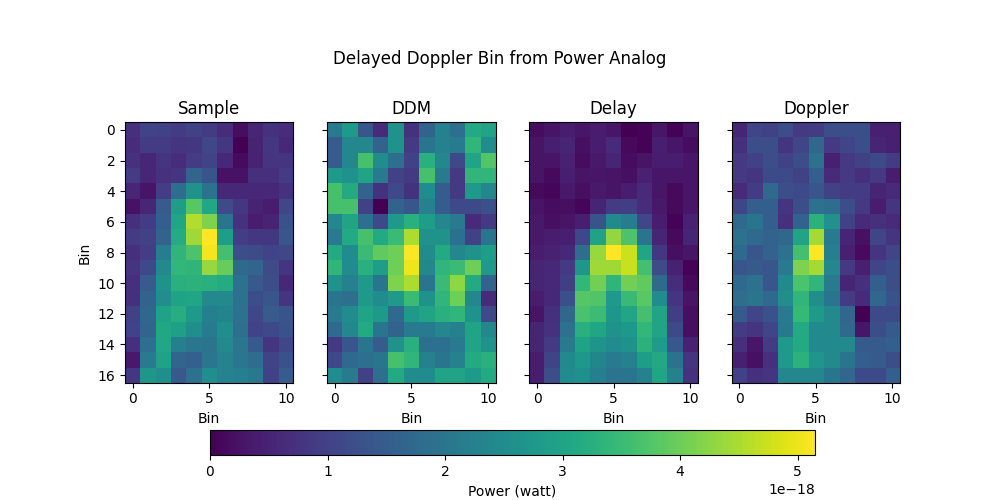
\includegraphics[width=0.75\textwidth]{Resource_PDFs/DDM.png}
    \caption{This is the delayed doppler map generated from the DDMI. This figure goes the raw sample, generated ddm, delay ddm, and doppler ddm of the analog power. The analog power is represents the true power that would have been measured \cite{Data}. Data provided from https://search.earthdata.nasa.gov/search/granules?p=C2146321631-POCLOUD.}
    \label{fig:Delayed Doppler Map}
\end{figure}

% ---------------- %

\section{Conclusion}
In conclusion the DDMI is a robust instrument. It allows for the real-time generation of DDM which permits the satellite to capture a greater number of samples. Working with modulated GPS signals, the DDMI and reduce the signal to noise ration (SNR) to extract the weak reflected GNSS signals. This also allows for monitoring using a range of GPS satellites. 

\clearpage
\appendix
\renewcommand{\theequation}{\thesection.\arabic{equation}}
\section{Instrumentation}

\setlength{\tabcolsep}{20pt}
\renewcommand{\arraystretch}{1.25}

\begin{table}[H]
    \centering
    \begin{tabular}{>{\bfseries}p{6cm} p{6cm}}
        \multicolumn{2}{c}{Delay Doppler Mapping Instrument (DDMI)} \\
        \hline
        Instrument Technology & GNSS receiver \\ 
        Resolution & 20-50 km \\
        Geometry & Push-broom scanning \\
        Waveband & 1.575 \\
        Data Format & NetCDF \\
        Data Access & Open \\
        \hline
    \end{tabular}
    \caption{This table was extracted from the CEOS handbook for the DDMI on board CYGNSS. Further information can be found here \cite{DDMI_Summary}.}
    \label{tab:DDMI_Summary}
\end{table}

% Sources
\clearpage
\printbibliography

\end{document}
